\documentclass[12pt,a4paper]{article}
\usepackage[utf8]{inputenc}
\usepackage[english]{babel}
\usepackage{amsmath}
\usepackage{amsfonts}
\usepackage{amssymb}
\usepackage{graphicx}
\usepackage{lmodern}
\usepackage[left=3cm,right=2cm,top=2cm,bottom=2cm]{geometry}
\begin{document}

\section*{Introduction}
The goal of this assignment is to use what we learn in the AI crash course.

\section{Machine Learning}

\subsection{Task}

The project of this part is to classify images of a well known MNIST dataset.

\subsection{Preprocessing}
We used cross-validation to create 3 subsets of our data.

Before applying ML algorithms, we have to preprocess our data. We used some techniques explained in the course but sometimes, techniques that we found online. We used PCA, T-SNE and Linear Discriminant Analysis (LDA).


You can see the 2D reduced space below for 2 algorithms.

\begin{figure}[h]
\centering
\includegraphics[scale=0.6]{fig/sphx_glr_plot_pca_vs_lda_001.png}
\end{figure}

\begin{figure}[h]
\centering
\includegraphics[scale=0.6]{fig/sphx_glr_plot_pca_vs_lda_002.png}
\end{figure}

\pagebreak

\subsection{Algorithms used}
We use common algorithm such as Random Forest, SVM which are well known algorithm and should work well with the dataset.

\subsection{Results}
Expectedly, we have pretty good result as you can see in the following figure for one algorithm.

\begin{figure}[h]
\centering
\includegraphics[scale=0.2]{fig/Good.png}
\caption{Confusion matrix with our Random Forest}
\end{figure}

\section{Deep Learning}

\subsection{Task}
Our task here is to classify images from a harder dataset.

\subsection{Preprocessing}
We also used cross-validation here.

In Deep Learning, the classification algorithm learn itself a representation of our data, so the previous pipeline and the current pipeline are a little bit different.

Our pre-processing was mainly dataset augmentation by rotating or translating images from our training set.

\subsection{Algorithms used}
To tackle this task, we mainly used CNN while changing the layers that composed our network.

\begin{figure}[h]
\centering
	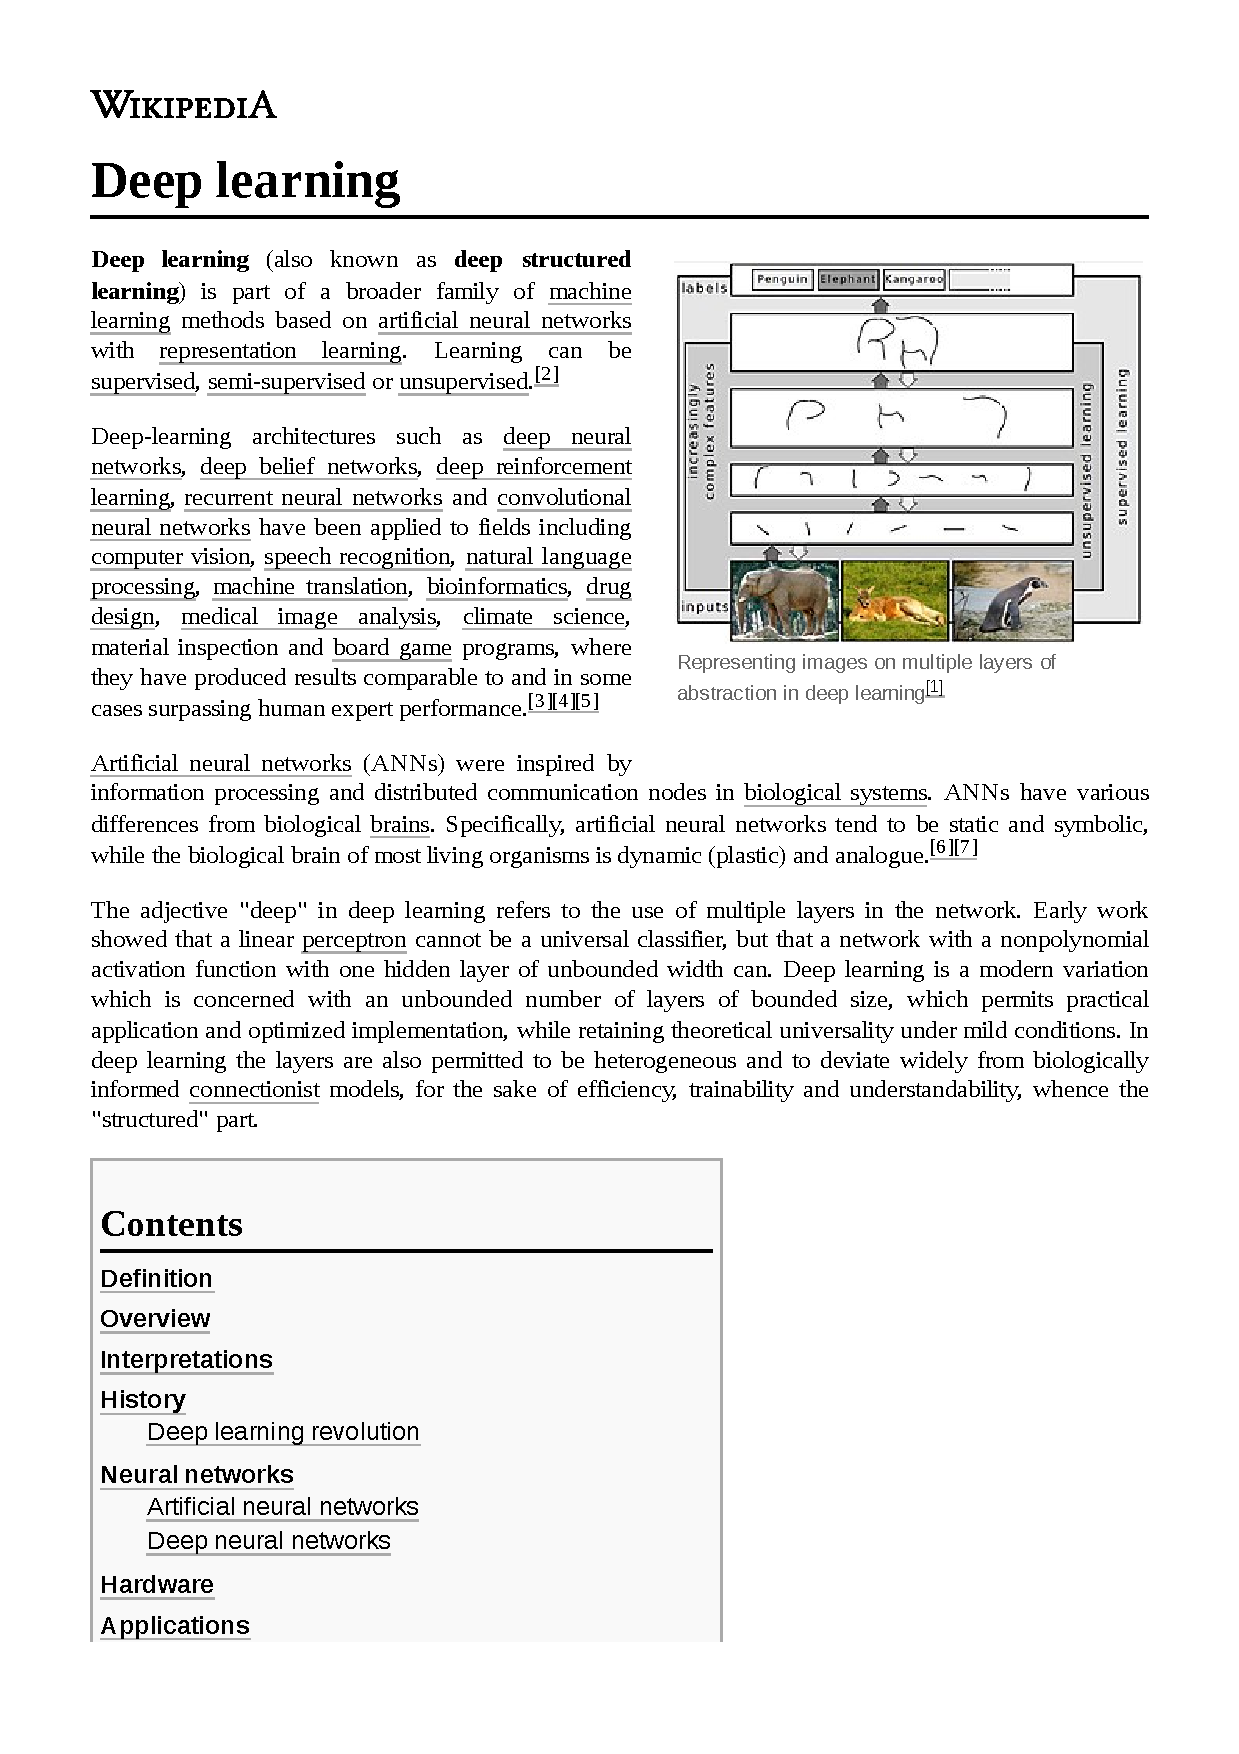
\includegraphics[scale=0.6]{courses/Deep_learning.pdf}
	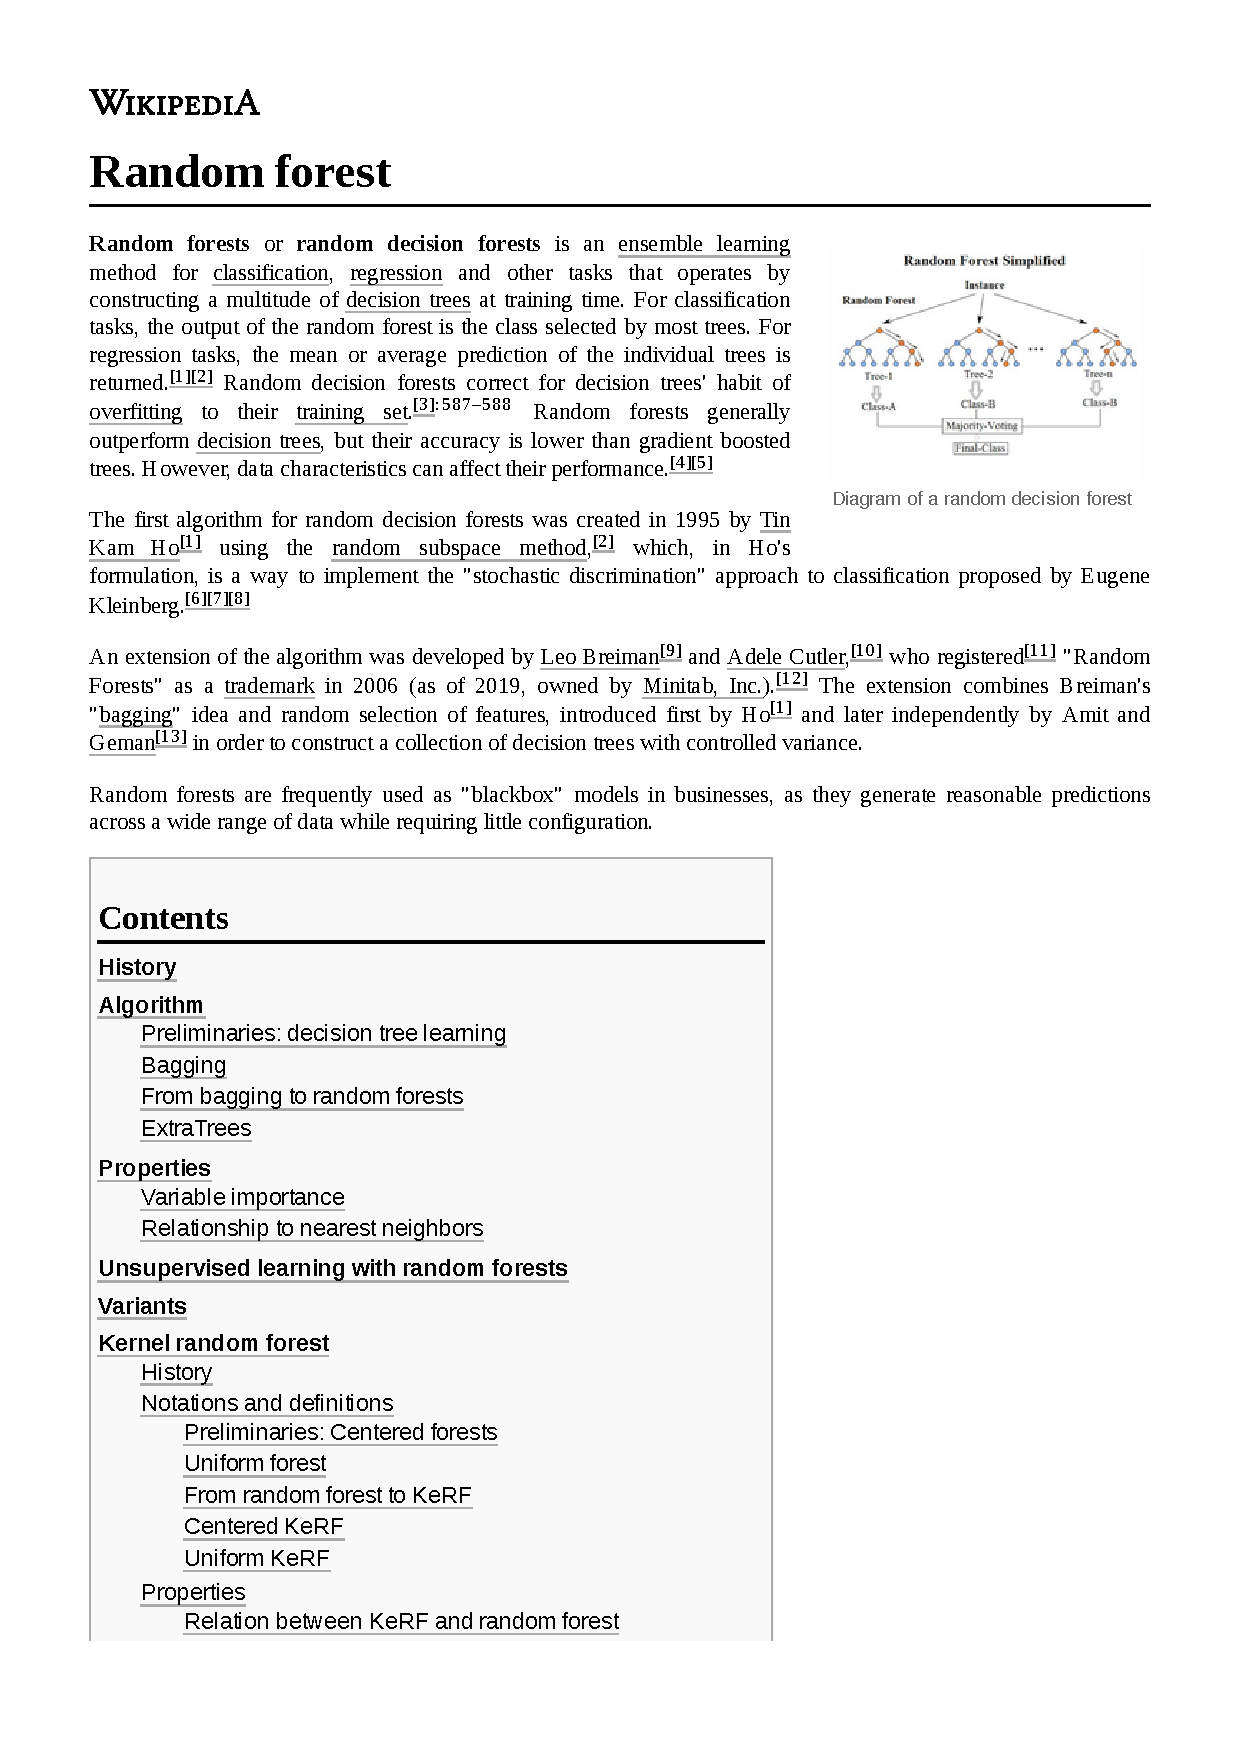
\includegraphics[scale=0.6]{courses/Random_forest.pdf}
	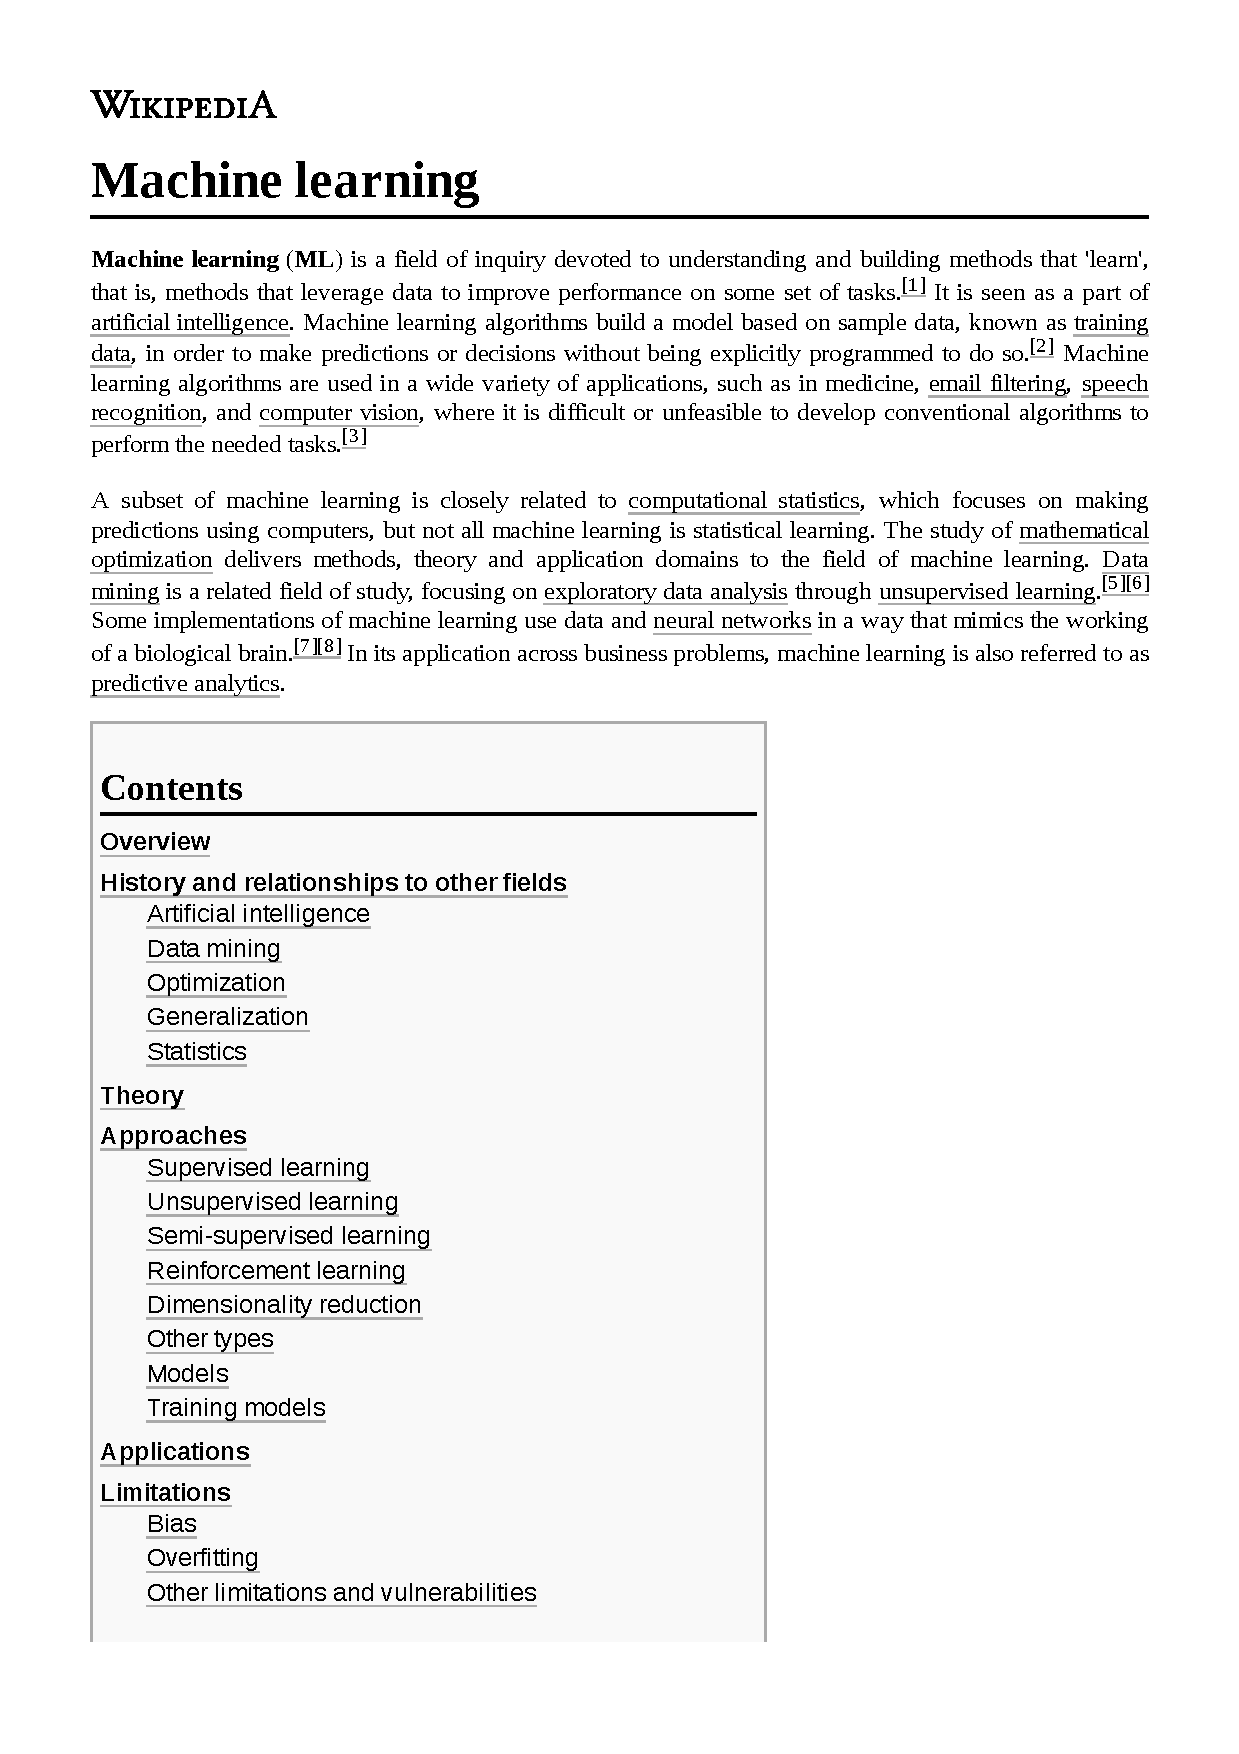
\includegraphics[scale=0.6]{courses/Machine_learning.pdf}
\end{figure}
\subsection{Results}

We have lower scores in this task than in the previous one. Not unexpected as the dataset is more complex and we did not train our CNN that much.

\begin{figure}[h]
\centering
\includegraphics[scale=0.2]{fig/Bad.png}
\caption{Confusion Matrix for a badly trained CNN}
\end{figure}

\end{document}
